\chapter{Análisis y Especificación del Sistema}
\label{cap:analisis}

Una vez establecida la metodología y la planificación del proyecto (capítulo~\ref{cap:metodologia}), este capítulo
formaliza el análisis del sistema desarrollado. Se identifican los actores, se derivan los requisitos
funcionales y no funcionales a partir de las Historias de Usuario gestionadas en el tablero,
se especifican los casos de uso del MVP y se establece la trazabilidad entre todos los artefactos.
Cierra el capítulo un modelo conceptual de dominio que abstrae las entidades principales del sistema,
dejando las decisiones de implementación para el capítulo de diseño (capítulo~\ref{cap:diseno-desarrollo}).

\section{Actores del Sistema}

El sistema reconoce tres actores primarios, que son las personas que lo utilizan, y dos actores
secundarios, servicios externos que no son humanos pero sin los cuales el sistema no puede completar sus
casos de uso principales.

El \textbf{Mayor Independiente} es la persona mayor que ha optado durante el \textit{onboarding} por
gestionar la aplicación por sí misma. Tiene acceso al chat por voz y a los ajustes de accesibilidad en su
propio dispositivo, y se autentica de forma anónima, de modo que su identidad queda ligada al terminal. El
\textbf{Mayor Vinculado} es aquel cuya configuración delega en un familiar: su interfaz se restringe al
chat por voz, en el llamado \textit{modo ultrasimple}, mientras el emparejamiento no se completa, y se
autentica igualmente de forma anónima. El \textbf{Familiar}, por último, es el adulto que asume la gestión
de la configuración del Mayor Vinculado, accede a un panel remoto desde su propio dispositivo y se
autentica con correo electrónico y contraseña, porque necesita una cuenta portable entre terminales.

En cuanto a los actores secundarios, la \textbf{API de Gemini} es el servicio al que se delega la
generación de las respuestas conversacionales, y la \textbf{API de Cloud Text-to-Speech} es la que
sintetiza la voz con la que esas respuestas se pronuncian. Aunque ninguno de los dos es un actor humano, su
consideración como actores del sistema es coherente con la práctica habitual en UML cuando un agente
externo dispara o atiende eventos del sistema. Ambos se consumen mediante llamadas a través de la red y
ambos condicionan la disponibilidad del caso de uso conversacional, tal y como recoge RNF-14.

Los dos perfiles de Mayor (Independiente y Vinculado) heredan del mismo concepto de usuario \textit{Mayor};
la diferencia entre ambos es de \textbf{configuración}, no de identidad, y se materializa en el
atributo \code{autonomy} del modelo de datos. Esta unificación es relevante para el diseño: una misma
jerarquía de pantallas y un mismo controlador atienden a ambos perfiles, alternando entre presentaciones
mediante un único condicional sobre \code{autonomy}.

\begin{figure}[htbp]
    \centering
    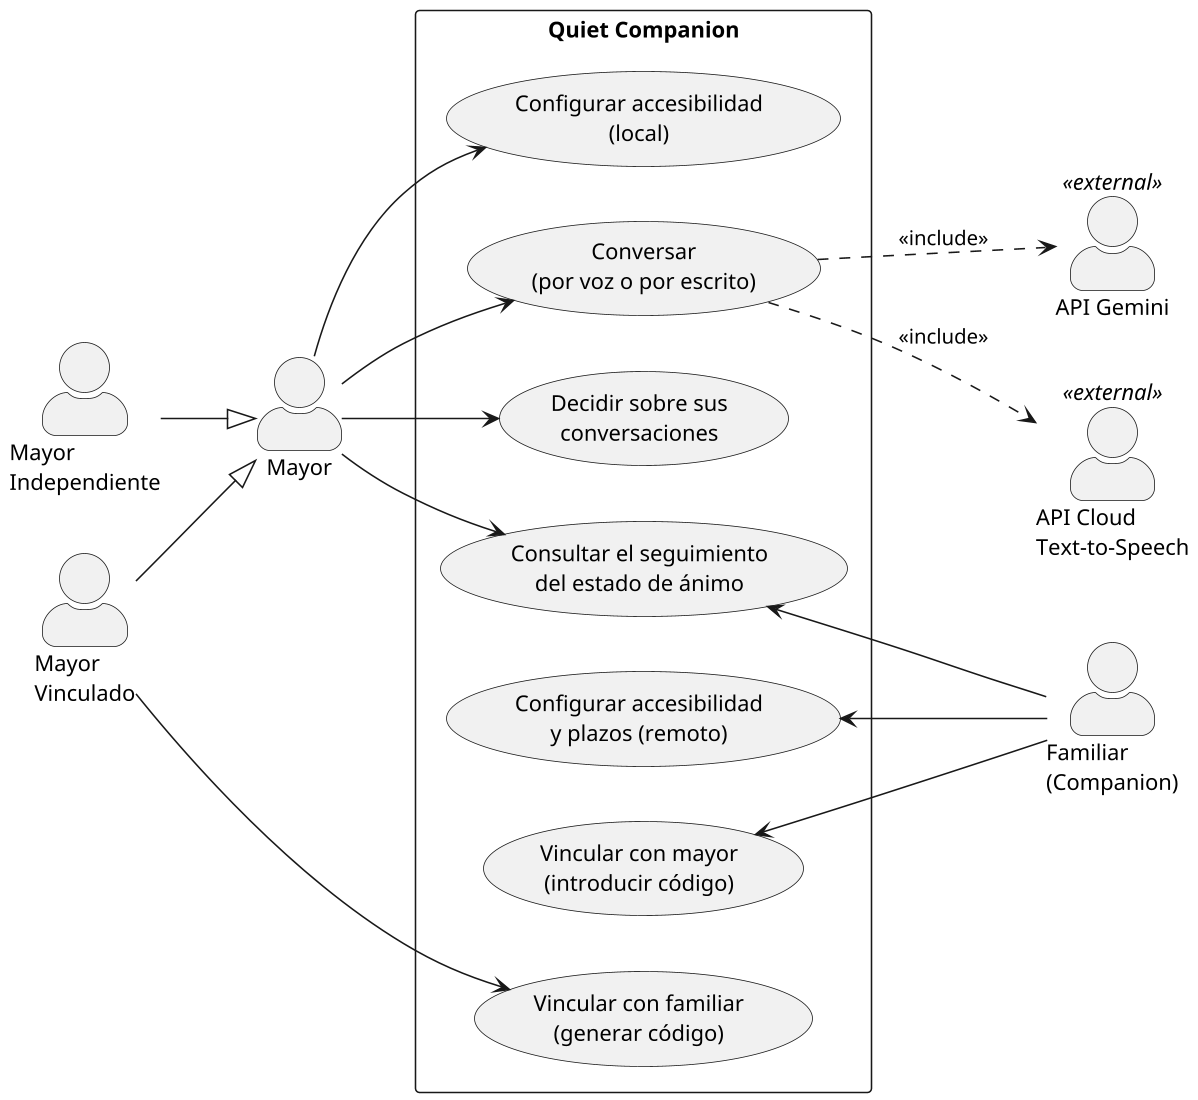
\includegraphics[width=0.8\textwidth]{imagenes/uml/diagrama_actores.png}
    \caption{Diagrama de actores del sistema.}
    \label{fig:actores}
\end{figure}

Este diagrama refleja la jerarquía de actores y las relaciones primarias con los casos de uso del MVP. La
especificación detallada de cada caso de uso se desarrolla en la Sección~\ref{sec:casos-de-uso}.

\section{Catálogo de requisitos}
Los requisitos se han derivado a partir de las Historias de Usuario (HU-1 a HU-6), las restricciones técnicas
declaradas por el análisis previo y los principios de diseño establecidos en el capítulo~\ref{cap:introduccion}. Se distinguen
\textbf{requisitos funcionales} (RF), que describen las capacidades del sistema, y \textbf{requisitos no
funcionales} (RNF), que describen las restricciones bajo las cuales esas capacidades deben cumplirse.

\subsection{Requisitos Funcionales}
Los requisitos funcionales se formalizan según una plantilla común: identificador, nombre, descripción,
entradas, salidas, prioridad e Historia de Usuario asociada.

\begin{table}[htbp]
    \centering
    \renewcommand{\arraystretch}{1.3}
    \begin{tabular}{|l|>{\raggedright\arraybackslash}p{0.72\textwidth}|}
        \hline
        \multicolumn{2}{|c|}{\textbf{Requisito Funcional: Selección Inicial de Modo de Uso}} \\
        \hline
        \textbf{ID} & RF-1 \\
        \hline
        \textbf{Origen} & HU-1 \\
        \hline
        \textbf{Prioridad} & Alta \\
        \hline
        \textbf{Descripción} & En el primer arranque, el sistema debe presentar al usuario dos opciones
            excluyentes, esto es, el modo independiente o la vinculación con un familiar, y configurar el perfil
            en función de la elección. \\
        \hline
        \textbf{Entradas} & Selección del usuario en la pantalla de onboarding. \\
        \hline
        \textbf{Salidas} & Perfil de usuario creado en la base de datos con \code{role = elder} y
            \code{autonomy} $\in$ \{\code{independent}, \code{dependent}\}. \\
        \hline
    \end{tabular}
    \caption{Requisito Funcional RF-1: Selección Inicial de Modo de Uso.}
    \label{tab:rf1}
\end{table}

\begin{table}[htbp]
    \centering
    \renewcommand{\arraystretch}{1.3}
    \begin{tabular}{|l|>{\raggedright\arraybackslash}p{0.72\textwidth}|}
        \hline
        \multicolumn{2}{|c|}{\textbf{Requisito Funcional: Generación y Consumo de Código de Vinculación}} \\
        \hline
        \textbf{ID} & RF-2 \\
        \hline
        \textbf{Origen} & HU-1 \\
        \hline
        \textbf{Prioridad} & Alta \\
        \hline
        \textbf{Descripción} & Si el mayor opta por el modo vinculado, el sistema debe generar un código
            corto de 4~caracteres en su dispositivo. El familiar, desde su propio dispositivo, debe poder
            introducir dicho código para completar el emparejamiento de forma atómica, sin que pueda
            quedar un estado intermedio en el que solo uno de los dos perfiles esté vinculado. \\
        \hline
        \textbf{Entradas} & Solicitud de generación de código (mayor) e introducción del código (familiar). \\
        \hline
        \textbf{Salidas} & Vinculación bidireccional persistida en la base de datos: el campo
            \code{linkedCompanionId} en el perfil del mayor y \code{linkedElderId} en el del familiar,
            ambos escritos dentro de una misma transacción. \\
        \hline
    \end{tabular}
    \caption{Requisito Funcional RF-2: Generación y Consumo de Código de Vinculación.}
    \label{tab:rf2}
\end{table}

\begin{table}[htbp]
    \centering
    \renewcommand{\arraystretch}{1.3}
    \begin{tabular}{|l|>{\raggedright\arraybackslash}p{0.72\textwidth}|}
        \hline
        \multicolumn{2}{|c|}{\textbf{Requisito Funcional: Procesamiento Conversacional por Voz}} \\
        \hline
        \textbf{ID} & RF-3 \\
        \hline
        \textbf{Origen} & HU-2 \\
        \hline
        \textbf{Prioridad} & Alta \\
        \hline
        \textbf{Descripción} & El sistema debe permitir al mayor mantener una
            conversación por voz pulsando un único botón central. La entrada de voz
            se transcribe a texto, se envía al modelo de lenguaje y la respuesta se
            reproduce mediante síntesis de voz. \\
        \hline
        \textbf{Entradas} & Pulsación del botón principal; señal de audio del usuario. \\
        \hline
        \textbf{Salidas} & Respuesta del asistente reproducida por audio y mostrada
            en pantalla con tipografía de gran tamaño. \\
        \hline
    \end{tabular}
    \caption{Requisito Funcional RF-3: Procesamiento Conversacional por Voz.}
    \label{tab:rf3}
\end{table}

\begin{table}[htbp]
    \centering
    \renewcommand{\arraystretch}{1.3}
    \begin{tabular}{|l|>{\raggedright\arraybackslash}p{0.72\textwidth}|}
        \hline
        \multicolumn{2}{|c|}{\textbf{Requisito Funcional: Indicación Visual del Estado del Asistente}} \\
        \hline
        \textbf{ID} & RF-4 \\
        \hline
        \textbf{Origen} & HU-2, HU-3 \\
        \hline
        \textbf{Prioridad} & Alta \\
        \hline
        \textbf{Descripción} & Durante una interacción de voz, el sistema debe comunicar visualmente en
            qué estado se encuentra, mediante las etiquetas «Te escucho», «Pensando» y «Respondiendo». La
            señalización debe ser perceptible por usuarios con limitaciones visuales moderadas y no puede
            descansar únicamente en el color. \\
        \hline
        \textbf{Entradas} & Cambios de estado internos del pipeline conversacional. \\
        \hline
        \textbf{Salidas} & Indicador visual y textual en pantalla. \\
        \hline
    \end{tabular}
    \caption{Requisito Funcional RF-4: Indicación Visual del Estado del Asistente.}
    \label{tab:rf4}
\end{table}

\begin{table}[htbp]
    \centering
    \renewcommand{\arraystretch}{1.3}
    \begin{tabular}{|l|>{\raggedright\arraybackslash}p{0.72\textwidth}|}
        \hline
        \multicolumn{2}{|c|}{\textbf{Requisito Funcional: Configuración de Parámetros de Accesibilidad}} \\
        \hline
        \textbf{ID} & RF-5 \\
        \hline
        \textbf{Origen} & HU-4 \\
        \hline
        \textbf{Prioridad} & Alta \\
        \hline
        \textbf{Descripción} & El sistema debe permitir configurar volumen de voz, velocidad de habla y
            tamaño del texto. El acceso depende del modo del mayor: si es independiente, accede desde su
            propio dispositivo; si está vinculado, la configuración se realiza únicamente desde el
            dispositivo del familiar. \\
        \hline
        \textbf{Entradas} & Valores de los parámetros configurables. \\
        \hline
        \textbf{Salidas} & Preferencias persistidas en la base de datos y aplicadas en la siguiente
            interacción del mayor. \\
        \hline
    \end{tabular}
    \caption{Requisito Funcional RF-5: Configuración de Parámetros de Accesibilidad.}
    \label{tab:rf5}
\end{table}

\begin{table}[htbp]
    \centering
    \renewcommand{\arraystretch}{1.3}
    \begin{tabular}{|l|>{\raggedright\arraybackslash}p{0.72\textwidth}|}
        \hline
        \multicolumn{2}{|c|}{\textbf{Requisito Funcional: Propagación Remota de la Configuración}} \\
        \hline
        \textbf{ID} & RF-6 \\
        \hline
        \textbf{Origen} & HU-4 \\
        \hline
        \textbf{Prioridad} & Alta \\
        \hline
        \textbf{Descripción} & Cuando el familiar modifica las preferencias del mayor desde su panel
            remoto, los cambios deben propagarse en tiempo real al dispositivo del mayor, sin requerir
            reinicio de la aplicación ni intervención por parte de éste. \\
        \hline
        \textbf{Entradas} & Modificación de preferencias en el panel del familiar. \\
        \hline
        \textbf{Salidas} & Actualización efectiva de los parámetros en el dispositivo del mayor. \\
        \hline
    \end{tabular}
    \caption{Requisito Funcional RF-6: Propagación Remota de la Configuración.}
    \label{tab:rf6}
\end{table}

\begin{table}[htbp]
    \centering
    \renewcommand{\arraystretch}{1.3}
    \begin{tabular}{|l|>{\raggedright\arraybackslash}p{0.72\textwidth}|}
        \hline
        \multicolumn{2}{|c|}{\textbf{Requisito Funcional: Memoria Conversacional Contextualizada}} \\
        \hline
        \textbf{ID} & RF-7 \\
        \hline
        \textbf{Origen} & HU-5 \\
        \hline
        \textbf{Prioridad} & Diferida a trabajo futuro \\
        \hline
        \textbf{Descripción} & El asistente debe inyectar en el contexto del modelo de lenguaje datos
            básicos del usuario (al menos su nombre) y un resumen del contexto reciente de conversaciones
            previas, de forma que las respuestas resulten personalizadas y coherentes con interacciones
            anteriores. \\
        \hline
        \textbf{Entradas} & Perfil del usuario y registro de conversaciones previas. \\
        \hline
        \textbf{Salidas} & Respuestas del asistente que reflejan el contexto personalizado del usuario. \\
        \hline
    \end{tabular}
    \caption{Requisito Funcional RF-7: Memoria Conversacional Contextualizada (diferido).}
    \label{tab:rf7}
\end{table}

\begin{table}[htbp]
    \centering
    \renewcommand{\arraystretch}{1.3}
    \begin{tabular}{|l|>{\raggedright\arraybackslash}p{0.72\textwidth}|}
        \hline
        \multicolumn{2}{|c|}{\textbf{Requisito Funcional: Catalogación Emocional de las Conversaciones}} \\
        \hline
        \textbf{ID} & RF-8 \\
        \hline
        \textbf{Origen} & HU-6 \\
        \hline
        \textbf{Prioridad} & Diferida a trabajo futuro \\
        \hline
        \textbf{Descripción} & Al finalizar una conversación, el sistema debe clasificar su sentimiento
            general (Positivo, Neutro o Negativo) y presentar el agregado en una vista accesible al mayor
            independiente y al familiar, según el modo. \\
        \hline
        \textbf{Entradas} & Transcripción de la conversación finalizada. \\
        \hline
        \textbf{Salidas} & Etiqueta de sentimiento almacenada y agregado visible en el panel de bienestar. \\
        \hline
    \end{tabular}
    \caption{Requisito Funcional RF-8: Catalogación Emocional de las Conversaciones (diferido).}
    \label{tab:rf8}
\end{table}

\subsection{Requisitos No Funcionales (RNF)}

Los requisitos no funcionales se agrupan en seis categorías canónicas. Aplican al sistema en su conjunto,
salvo indicación contraria.

\paragraph{Usabilidad y accesibilidad}
\begin{itemize}
    \item \textbf{RNF-1. Cumplimiento WCAG~2.2.} La interfaz dirigida al mayor debe cumplir los criterios
    de éxito de nivel~AA de la norma WCAG~2.2, en particular los relativos a perceptibilidad (contraste,
    tamaño de texto) y operabilidad (área activa de elementos táctiles, ausencia de gestos complejos).
    \item \textbf{RNF-2. Áreas táctiles mínimas.} Todo elemento interactivo de la interfaz del mayor debe
    tener un área activa de al menos $80 \times 80$ píxeles lógicos.
    \item \textbf{RNF-3. Tipografías mínimas.} El texto de cuerpo en la interfaz del mayor debe
    presentarse a un tamaño mínimo de 20~sp y los títulos a un mínimo de 28~sp, sujetos al multiplicador
    definido por el usuario en sus preferencias.
    \item \textbf{RNF-4. Interacciones simples.} La interfaz del mayor debe operarse exclusivamente
    mediante pulsación simple, excluyéndose el doble toque, la pulsación prolongada y los gestos de
    deslizamiento.
    \item \textbf{RNF-5. Idioma.} Todos los textos de la interfaz, así como las entradas y salidas de
    voz, deben presentarse en español de España (es-ES).
\end{itemize}

\paragraph{Rendimiento}
\begin{itemize}
    \item \textbf{RNF-6. Plataforma objetivo.} El sistema debe ejecutarse correctamente en dispositivos
    Android con \code{minSdk = 24} (Android~7.0), lo que asegura compatibilidad con terminales de gama
    media-baja desde 2016.
    \item \textbf{RNF-7. Latencia de respuesta conversacional.} La latencia percibida entre el fin de la
    entrada de voz del usuario y el inicio de la respuesta sintetizada no debería superar los 5~segundos
    en condiciones normales de red.
    % **NOTE: confirmar umbral con pruebas en dispositivo real antes de la entrega; ajustar si las mediciones lo desmienten.
\end{itemize}

\paragraph{Seguridad}
\begin{itemize}
    \item \textbf{RNF-8. Protección de credenciales de servicios externos.} Las claves de API de servicios
    externos (en particular la clave de la API de Gemini) no deben residir en el binario distribuido al
    usuario. Actualmente la clave se gestiona vía \code{flutter\_dotenv} en desarrollo; está prevista la
    migración a Cloud Functions de Firebase para producción, de modo que el cliente nunca acceda
    directamente al LLM.
    \item \textbf{RNF-9. Aislamiento de identidades.} Las operaciones de escritura que afecten a documentos
    de un usuario distinto del autenticado, señaladamente el emparejamiento entre el mayor y el familiar,
    deben ejecutarse desde un entorno servidor de confianza y no desde el cliente. El requisito quedó
    cubierto al trasladar la vinculación a una función en la nube, según se documenta en el
    capítulo~\ref{cap:diseno-desarrollo}.
\end{itemize}

\paragraph{Privacidad y protección de datos}
\begin{itemize}
    \item \textbf{RNF-10. Tratamiento de datos personales.} El sistema procesa datos de carácter personal
    (identificadores anónimos, preferencias del usuario y, en futuras versiones, transcripciones
    conversacionales y categorizaciones emocionales). Su tratamiento se ajustará al Reglamento General de
    Protección de Datos (Reglamento UE 2016/679, RGPD), aplicando los principios de minimización de datos,
    limitación de la finalidad y limitación del plazo de conservación. El registro de conversaciones, cuando
    se implemente, se gobernará por consentimiento explícito (\textit{opt-in}) desactivado por defecto, y
    será controlable por el mayor o por el familiar gestor.
    % **NOTE: pendiente de formalización completa una vez se implementen HU-5 y HU-6; documentar base legal, periodos de retención y procedimiento de derecho de borrado.
\end{itemize}

\paragraph{Mantenibilidad}
\begin{itemize}
    \item \textbf{RNF-11. Arquitectura.} El código fuente debe organizarse según el modelo Clean
    Architecture combinado con Feature-Sliced Design (CFS), con separación estricta entre las capas de
    presentación, dominio y datos, y sin acoplamiento horizontal entre features.
    \item \textbf{RNF-12. Inyección de dependencias.} Los servicios externos y repositorios deben
    inyectarse en los controladores mediante el sistema de providers de Riverpod, evitando instanciación
    directa dentro de la lógica de negocio.
    \item \textbf{RNF-13. Calidad estática.} Todo módulo modificado debe superar el análisis estático
    (\code{flutter analyze}) sin advertencias antes de su integración en la rama principal.
\end{itemize}

\paragraph{Disponibilidad}
\begin{itemize}
    \item \textbf{RNF-14. Dependencia de conectividad.} El sistema requiere conexión a internet para las
    funcionalidades conversacionales (acceso a la API de Gemini) y de sincronización (acceso a Firestore).
    Ante pérdida de conectividad, el sistema debe degradarse de forma controlada, informando al usuario de
    la indisponibilidad temporal en lugar de fallar silenciosamente.
    % **NOTE: definir comportamiento concreto en pantalla durante la fase de pulido de UX.
\end{itemize}

\section{Casos de Uso}
\label{sec:casos-de-uso}
Esta sección formaliza los casos de uso del MVP estabilizado (HU-1 a HU-4). Las HU diferidas
(HU-5 y HU-6) no se especifican aquí; quedan documentadas en el capítulo~\ref{cap:desarrollo-futuro} como líneas de trabajo
futuro.

\subsection{Diagramas de casos de uso (UML)}

\begin{figure}[htbp]
    \centering
    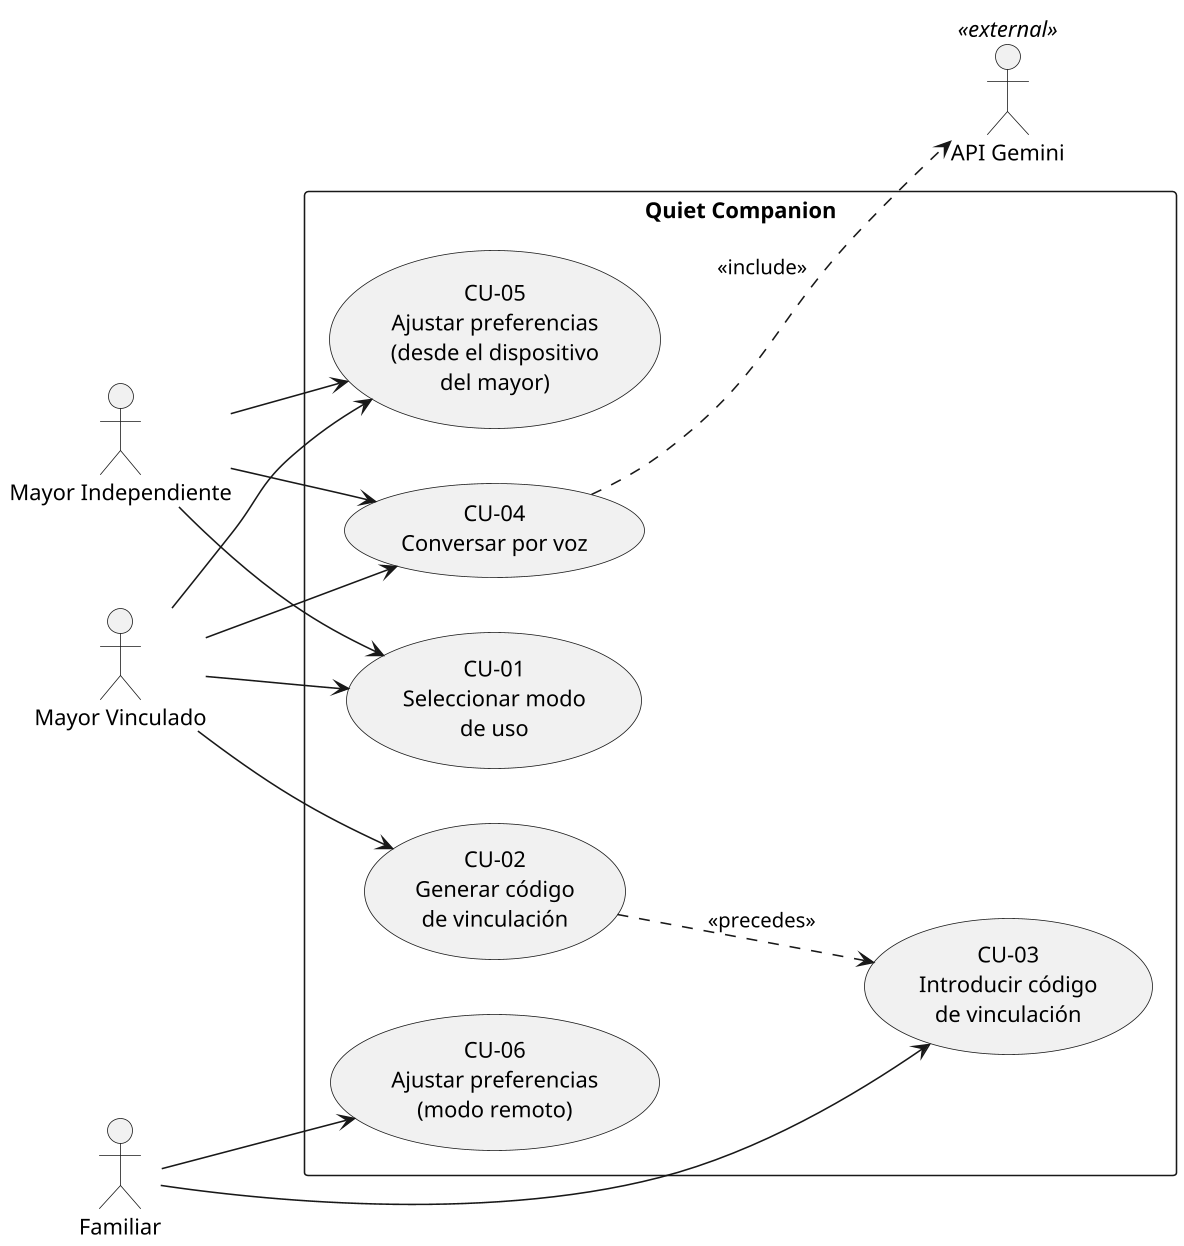
\includegraphics[width=0.8\textwidth]{imagenes/uml/diagrama_casos_de_uso.png}
    \caption{Diagrama de casos de uso del MVP.}
    \label{fig:casos-de-uso}
\end{figure}

\subsection{Especificación detallada}

Cada caso de uso se documenta según la plantilla: identificador, nombre, actor primario,
precondiciones, flujo principal, flujos alternativos y postcondiciones.

\paragraph{CU-01. Seleccionar modo de uso}

\noindent\textbf{Actor primario:} Mayor (Independiente o Vinculado, según resultado del caso).

\noindent\textbf{Precondiciones:} Es el primer arranque de la aplicación en el dispositivo, o el usuario
ha solicitado expresamente reiniciar su perfil.

\noindent\textbf{Flujo principal:}
\begin{enumerate}[nosep]
    \item El sistema presenta una pantalla con dos botones de gran tamaño: \textit{«Voy a configurar mi
    aplicación»} y \textit{«Un familiar me va a ayudar»}.
    \item El usuario pulsa una de las dos opciones.
    \item El sistema crea un perfil anónimo en la base de datos con \code{role = elder}.
    \item Si la opción seleccionada es la primera, el sistema asigna \code{autonomy = independent} y
    redirige a la pantalla principal con acceso a los ajustes habilitado.
    \item Si la opción seleccionada es la segunda, el sistema asigna \code{autonomy = dependent} y
    desencadena el caso de uso CU-02.
\end{enumerate}

\noindent\textbf{Flujos alternativos:} Ninguno relevante para el MVP.

\noindent\textbf{Postcondiciones:} Existe un perfil de mayor en la base de datos con su \code{autonomy}
definida.

\bigskip

\paragraph{CU-02. Generar código de vinculación}

\noindent\textbf{Actor primario:} Mayor Vinculado.

\noindent\textbf{Precondiciones:} Se ha completado CU-01 con \code{autonomy = dependent}.

\noindent\textbf{Flujo principal:}
\begin{enumerate}[nosep]
    \item El sistema genera un código aleatorio de 4~caracteres (alfanumérico, excluidos caracteres
    confundibles: O e I).
    \item El sistema persiste el código en el perfil del mayor y lo presenta en pantalla con tipografía de
    gran tamaño.
    \item La interfaz del mayor permanece bloqueada en modo ultrasimple mientras el campo
    \code{linkedCompanionId} sea nulo.
\end{enumerate}

\noindent\textbf{Flujos alternativos:} El alfabeto empleado ofrece unas 923.000 combinaciones posibles y el
sistema no reintenta la generación ante una eventual colisión. Es una limitación conocida y asumida a la
escala de pruebas del MVP, que se documenta como deuda en el capítulo~\ref{cap:diseno-desarrollo}.

\noindent\textbf{Postcondiciones:} Existe un código de vinculación activo en el perfil del mayor,
pendiente de ser consumido por un familiar.

\bigskip

\paragraph{CU-03. Introducir código de vinculación}

\noindent\textbf{Actor primario:} Familiar.

\noindent\textbf{Precondiciones:} El familiar tiene una cuenta autenticada (correo + contraseña) y
posee un código de vinculación válido proporcionado por el mayor.

\noindent\textbf{Flujo principal:}
\begin{enumerate}[nosep]
    \item El familiar accede a la pantalla de emparejamiento desde su dispositivo.
    \item El familiar introduce el código de 4~caracteres.
    \item El sistema valida en el servidor que el código existe y no ha sido consumido, y comprueba que
    quien solicita la vinculación es efectivamente un familiar registrado.
    \item El sistema ejecuta una operación atómica que actualiza, en una misma transacción, el campo
    \code{linkedCompanionId} del mayor y el campo \code{linkedElderId} del familiar, y consume el código
    para que no pueda reutilizarse.
    \item El sistema notifica el emparejamiento exitoso al familiar y desbloquea automáticamente la
    interfaz del mayor.
\end{enumerate}

\noindent\textbf{Flujos alternativos:}
\begin{itemize}[nosep]
    \item \textbf{3a.} Código inexistente o ya consumido: el sistema muestra mensaje de error y permite
    reintentar.
\end{itemize}

\noindent\textbf{Postcondiciones:} Los perfiles de mayor y familiar están vinculados de forma
bidireccional y el código ha quedado consumido. La interfaz del mayor sale del modo ultrasimple sin que
éste tenga que intervenir.

\bigskip

\paragraph{CU-04. Conversar por voz}

\noindent\textbf{Actor primario:} Mayor (cualquier modalidad).

\noindent\textbf{Actor secundario:} API de Gemini.

\noindent\textbf{Precondiciones:} El mayor tiene un perfil activo. El dispositivo dispone de conexión a
internet y de permisos de micrófono concedidos.

\noindent\textbf{Flujo principal:}
\begin{enumerate}[nosep]
    \item El mayor pulsa el botón central de micrófono en la pantalla principal.
    \item El sistema solicita permiso de micrófono si no estaba ya concedido y comienza la captura de
    audio. La interfaz indica visualmente el estado mediante la etiqueta «Te escucho».
    \item El sistema transcribe el audio a texto mediante el servicio de reconocimiento de voz
    (locale \code{es-ES}).
    \item El sistema cambia el estado a «Pensando» y envía el texto transcrito a la API de Gemini, junto
    con el \code{systemInstruction} configurado.
    \item La API de Gemini devuelve una respuesta textual.
    \item El sistema cambia el estado a «Respondiendo», muestra el texto de la respuesta en pantalla con
    tipografía de gran tamaño y lo reproduce mediante síntesis de voz, aplicando los parámetros del usuario
    (\code{volume} y \code{speechRate}). Si la síntesis en la nube no está disponible, la respuesta se
    pronuncia con el motor de voz del propio dispositivo.
    \item Al finalizar la reproducción, el sistema vuelve al estado de reposo.
\end{enumerate}

\noindent\textbf{Flujos alternativos:}
\begin{itemize}[nosep]
    \item \textbf{2a.} Permiso de micrófono denegado: el sistema informa al usuario de la imposibilidad
    de proceder y cancela la operación.
    \item \textbf{4a.} Error de red o error en la respuesta de la API: el sistema vuelve al estado de
    reposo e informa con un mensaje accesible.
    % **NOTE: definir mensaje y comportamiento concreto durante el pulido de UX.
\end{itemize}

\noindent\textbf{Postcondiciones:} La interacción se ha completado o cancelado de forma controlada.

\bigskip

\paragraph{CU-05. Ajustar preferencias (modo independiente)}

\noindent\textbf{Actor primario:} Mayor Independiente.

\noindent\textbf{Precondiciones:} El mayor tiene un perfil con \code{autonomy = independent}.

\noindent\textbf{Flujo principal:}
\begin{enumerate}[nosep]
    \item El mayor accede a la pantalla de ajustes desde la pantalla principal.
    \item El sistema muestra los controles de volumen, velocidad de voz y tamaño de texto, presentados
    como botones grandes (incremento / decremento), no como sliders deslizables.
    \item El mayor modifica uno o varios parámetros.
    \item Cada cambio se persiste en la base de datos al soltar el control.
    \item Los nuevos parámetros se aplican inmediatamente a las próximas interacciones de voz y al
    renderizado de la interfaz.
\end{enumerate}

\noindent\textbf{Flujos alternativos:} Ninguno relevante.

\noindent\textbf{Postcondiciones:} Las preferencias del mayor están actualizadas y aplicadas.

\bigskip

\paragraph{CU-06. Ajustar preferencias (modo remoto, desde el Familiar)}

\noindent\textbf{Actor primario:} Familiar.

\noindent\textbf{Precondiciones:} El familiar está vinculado a un mayor, es decir, existen
\code{linkedElderId} en su perfil y \code{linkedCompanionId} en el del mayor.

\noindent\textbf{Flujo principal:}
\begin{enumerate}[nosep]
    \item El familiar accede al panel remoto desde su dispositivo.
    \item El sistema muestra los controles de configuración con el estado actual de las preferencias del
    mayor.
    \item El familiar modifica uno o varios parámetros.
    \item Al finalizar el ajuste de cada control, el cambio se persiste en la base de datos.
    \item El cambio se propaga en tiempo real al dispositivo del mayor mediante la suscripción reactiva a
    su documento de usuario, sin que el mayor deba intervenir.
\end{enumerate}

\noindent\textbf{Flujos alternativos:}
\begin{itemize}[nosep]
    \item \textbf{4a.} Error de persistencia: el sistema revierte el control a su valor anterior y
    notifica el fallo al familiar.
\end{itemize}

\noindent\textbf{Postcondiciones:} Las preferencias del mayor están actualizadas y aplicadas en su
dispositivo.

\subsection{Trazabilidad}

La siguiente tabla cruza Historias de Usuario, Requisitos Funcionales y Casos de Uso. Permite verificar
que cada artefacto de análisis tiene origen en una necesidad real del usuario y, recíprocamente, que toda
HU del MVP estabilizado se ha traducido en al menos un caso de uso especificado.

\begin{table}[htbp]
    \centering
    \begin{tabularx}{\textwidth}{@{}c >{\RaggedRight\arraybackslash}X >{\RaggedRight\arraybackslash}X@{}}
        \toprule
        \textbf{Historia de Usuario} & \textbf{Requisitos Funcionales} & \textbf{Casos de Uso} \\
        \midrule
        HU-1 & RF-1, RF-2                & CU-01, CU-02, CU-03 \\
        HU-2 & RF-3, RF-4                & CU-04 \\
        HU-3 & No procede                & No procede \\
        HU-4 & RF-5, RF-6                & CU-05, CU-06 \\
        HU-5 & RF-7 (diferido)           & No procede \\
        HU-6 & RF-8 (diferido)           & No procede \\
        \bottomrule
    \end{tabularx}
    \caption{Trazabilidad entre Historias de Usuario, Requisitos Funcionales y Casos de Uso.}
    \label{tab:trazabilidad}
\end{table}

HU-3 no genera casos de uso propios porque sus criterios son restricciones transversales de accesibilidad
que se materializan como RNF y como condiciones de diseño aplicables a todos los casos de uso. Esta
decisión es deliberada y evita la duplicación que se produciría al crear casos de uso ficticios para una
HU de naturaleza no funcional.

\section{Modelo conceptual de dominio}

El modelo conceptual identifica las entidades principales que el sistema manipula y las relaciones entre
ellas, con independencia de las decisiones tecnológicas de implementación.

El sistema manipula tres entidades. El \textbf{Usuario} representa a una persona que interactúa con el
sistema; tiene un rol, que puede ser \textit{Mayor} o \textit{Familiar}, y, en el caso del mayor, un grado
de autonomía que distingue al independiente del vinculado. Las \textbf{Preferencias} son el conjunto de
parámetros de accesibilidad asociados a un usuario mayor, esto es, el volumen de la voz, la velocidad del
habla y el multiplicador del tamaño de texto. La \textbf{Conversación}, por último, representa una
interacción de voz entre el mayor y el asistente, con sus transcripciones, las respuestas generadas y los
metadatos de la sesión; se incluye en el modelo porque el dominio la contiene, aunque su persistencia
corresponde a HU-5 y no forma parte del MVP entregado.
% **NOTE: la entidad Conversación queda en el modelo conceptual pero sin implementar (HU-5, HU-6).

La relación principal es la \textbf{vinculación} entre un mayor y un familiar. Es binaria, bidireccional y
opcional, se establece mediante un código temporal de un solo uso y, una vez establecida, autoriza al
familiar a leer el perfil del mayor y a modificar sus preferencias, y solo esas.

\begin{figure}[htbp]
    \centering
    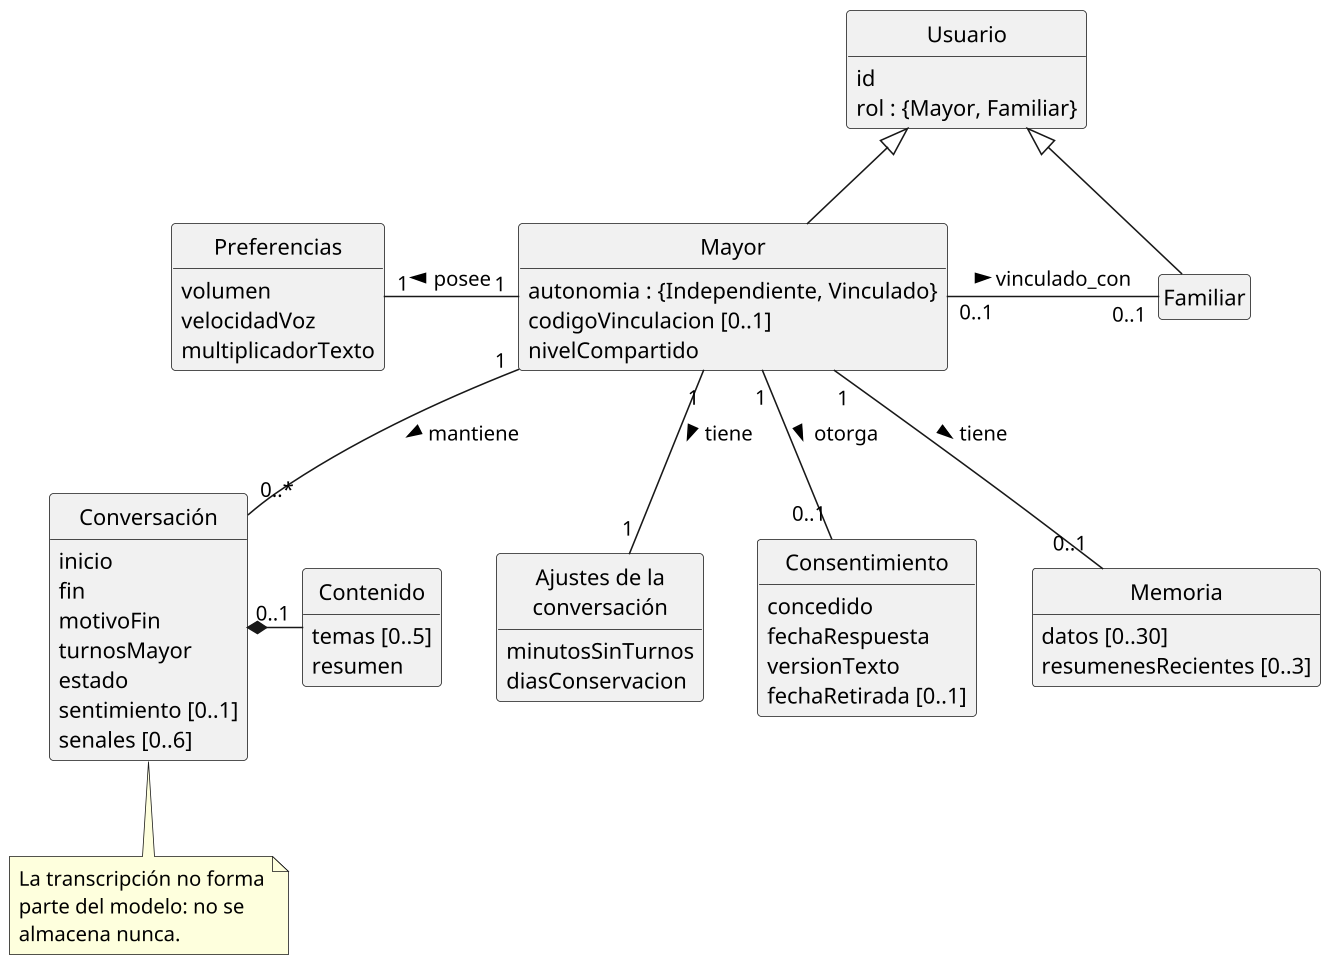
\includegraphics[width=0.8\textwidth]{imagenes/uml/diagrama_conceptual.png}
    \caption{Modelo conceptual de dominio del sistema.}
    \label{fig:dominio}
\end{figure}

La cardinalidad $0..1$ en ambos extremos de la relación \textit{vinculado\_con} refleja una decisión de
diseño relevante: un mayor solo puede estar vinculado a un familiar y viceversa. Esta restricción
simplifica el modelo y respeta la naturaleza personal del vínculo de cuidado. En extensiones futuras
(por ejemplo, varios familiares supervisando a un mismo mayor) la cardinalidad se ampliaría a $0..n$
en el lado del Familiar.
